\documentclass[1p]{elsarticle_modified}
%\bibliographystyle{elsarticle-num}

%\usepackage[colorlinks]{hyperref}
%\usepackage{abbrmath_seonhwa} %\Abb, \Ascr, \Acal ,\Abf, \Afrak
\usepackage{amsfonts}
\usepackage{amssymb}
\usepackage{amsmath}
\usepackage{amsthm}
\usepackage{scalefnt}
\usepackage{amsbsy}
\usepackage{kotex}
\usepackage{caption}
\usepackage{subfig}
\usepackage{color}
\usepackage{graphicx}
\usepackage{xcolor} %% white, black, red, green, blue, cyan, magenta, yellow
\usepackage{float}
\usepackage{setspace}
\usepackage{hyperref}

\usepackage{tikz}
\usetikzlibrary{arrows}

\usepackage{multirow}
\usepackage{array} % fixed length table
\usepackage{hhline}

%%%%%%%%%%%%%%%%%%%%%
\makeatletter
\renewcommand*\env@matrix[1][\arraystretch]{%
	\edef\arraystretch{#1}%
	\hskip -\arraycolsep
	\let\@ifnextchar\new@ifnextchar
	\array{*\c@MaxMatrixCols c}}
\makeatother %https://tex.stackexchange.com/questions/14071/how-can-i-increase-the-line-spacing-in-a-matrix
%%%%%%%%%%%%%%%

\usepackage[normalem]{ulem}

\newcommand{\msout}[1]{\ifmmode\text{\sout{\ensuremath{#1}}}\else\sout{#1}\fi}
%SOURCE: \msout is \stkout macro in https://tex.stackexchange.com/questions/20609/strikeout-in-math-mode

\newcommand{\cancel}[1]{
	\ifmmode
	{\color{red}\msout{#1}}
	\else
	{\color{red}\sout{#1}}
	\fi
}

\newcommand{\add}[1]{
	{\color{blue}\uwave{#1}}
}

\newcommand{\replace}[2]{
	\ifmmode
	{\color{red}\msout{#1}}{\color{blue}\uwave{#2}}
	\else
	{\color{red}\sout{#1}}{\color{blue}\uwave{#2}}
	\fi
}

\newcommand{\Sol}{\mathcal{S}} %segment
\newcommand{\D}{D} %diagram
\newcommand{\A}{\mathcal{A}} %arc


%%%%%%%%%%%%%%%%%%%%%%%%%%%%%5 test

\def\sl{\operatorname{\textup{SL}}(2,\Cbb)}
\def\psl{\operatorname{\textup{PSL}}(2,\Cbb)}
\def\quan{\mkern 1mu \triangleright \mkern 1mu}

\theoremstyle{definition}
\newtheorem{thm}{Theorem}[section]
\newtheorem{prop}[thm]{Proposition}
\newtheorem{lem}[thm]{Lemma}
\newtheorem{ques}[thm]{Question}
\newtheorem{cor}[thm]{Corollary}
\newtheorem{defn}[thm]{Definition}
\newtheorem{exam}[thm]{Example}
\newtheorem{rmk}[thm]{Remark}
\newtheorem{alg}[thm]{Algorithm}

\newcommand{\I}{\sqrt{-1}}
\begin{document}

%\begin{frontmatter}
%
%\title{Boundary parabolic representations of knots up to 8 crossings}
%
%%% Group authors per affiliation:
%\author{Yunhi Cho} 
%\address{Department of Mathematics, University of Seoul, Seoul, Korea}
%\ead{yhcho@uos.ac.kr}
%
%
%\author{Seonhwa Kim} %\fnref{s_kim}}
%\address{Center for Geometry and Physics, Institute for Basic Science, Pohang, 37673, Korea}
%\ead{ryeona17@ibs.re.kr}
%
%\author{Hyuk Kim}
%\address{Department of Mathematical Sciences, Seoul National University, Seoul 08826, Korea}
%\ead{hyukkim@snu.ac.kr}
%
%\author{Seokbeom Yoon}
%\address{Department of Mathematical Sciences, Seoul National University, Seoul, 08826,  Korea}
%\ead{sbyoon15@snu.ac.kr}
%
%\begin{abstract}
%We find all boundary parabolic representation of knots up to 8 crossings.
%
%\end{abstract}
%\begin{keyword}
%    \MSC[2010] 57M25 
%\end{keyword}
%
%\end{frontmatter}

%\linenumbers
%\tableofcontents
%
\newcommand\colored[1]{\textcolor{white}{\rule[-0.35ex]{0.8em}{1.4ex}}\kern-0.8em\color{red} #1}%
%\newcommand\colored[1]{\textcolor{white}{ #1}\kern-2.17ex	\textcolor{white}{ #1}\kern-1.81ex	\textcolor{white}{ #1}\kern-2.15ex\color{red}#1	}

{\Large $\underline{12n_{0276}~(K12n_{0276})}$}

\setlength{\tabcolsep}{10pt}
\renewcommand{\arraystretch}{1.6}
\vspace{1cm}\begin{tabular}{m{100pt}>{\centering\arraybackslash}m{274pt}}
\multirow{5}{120pt}{
	\centering
	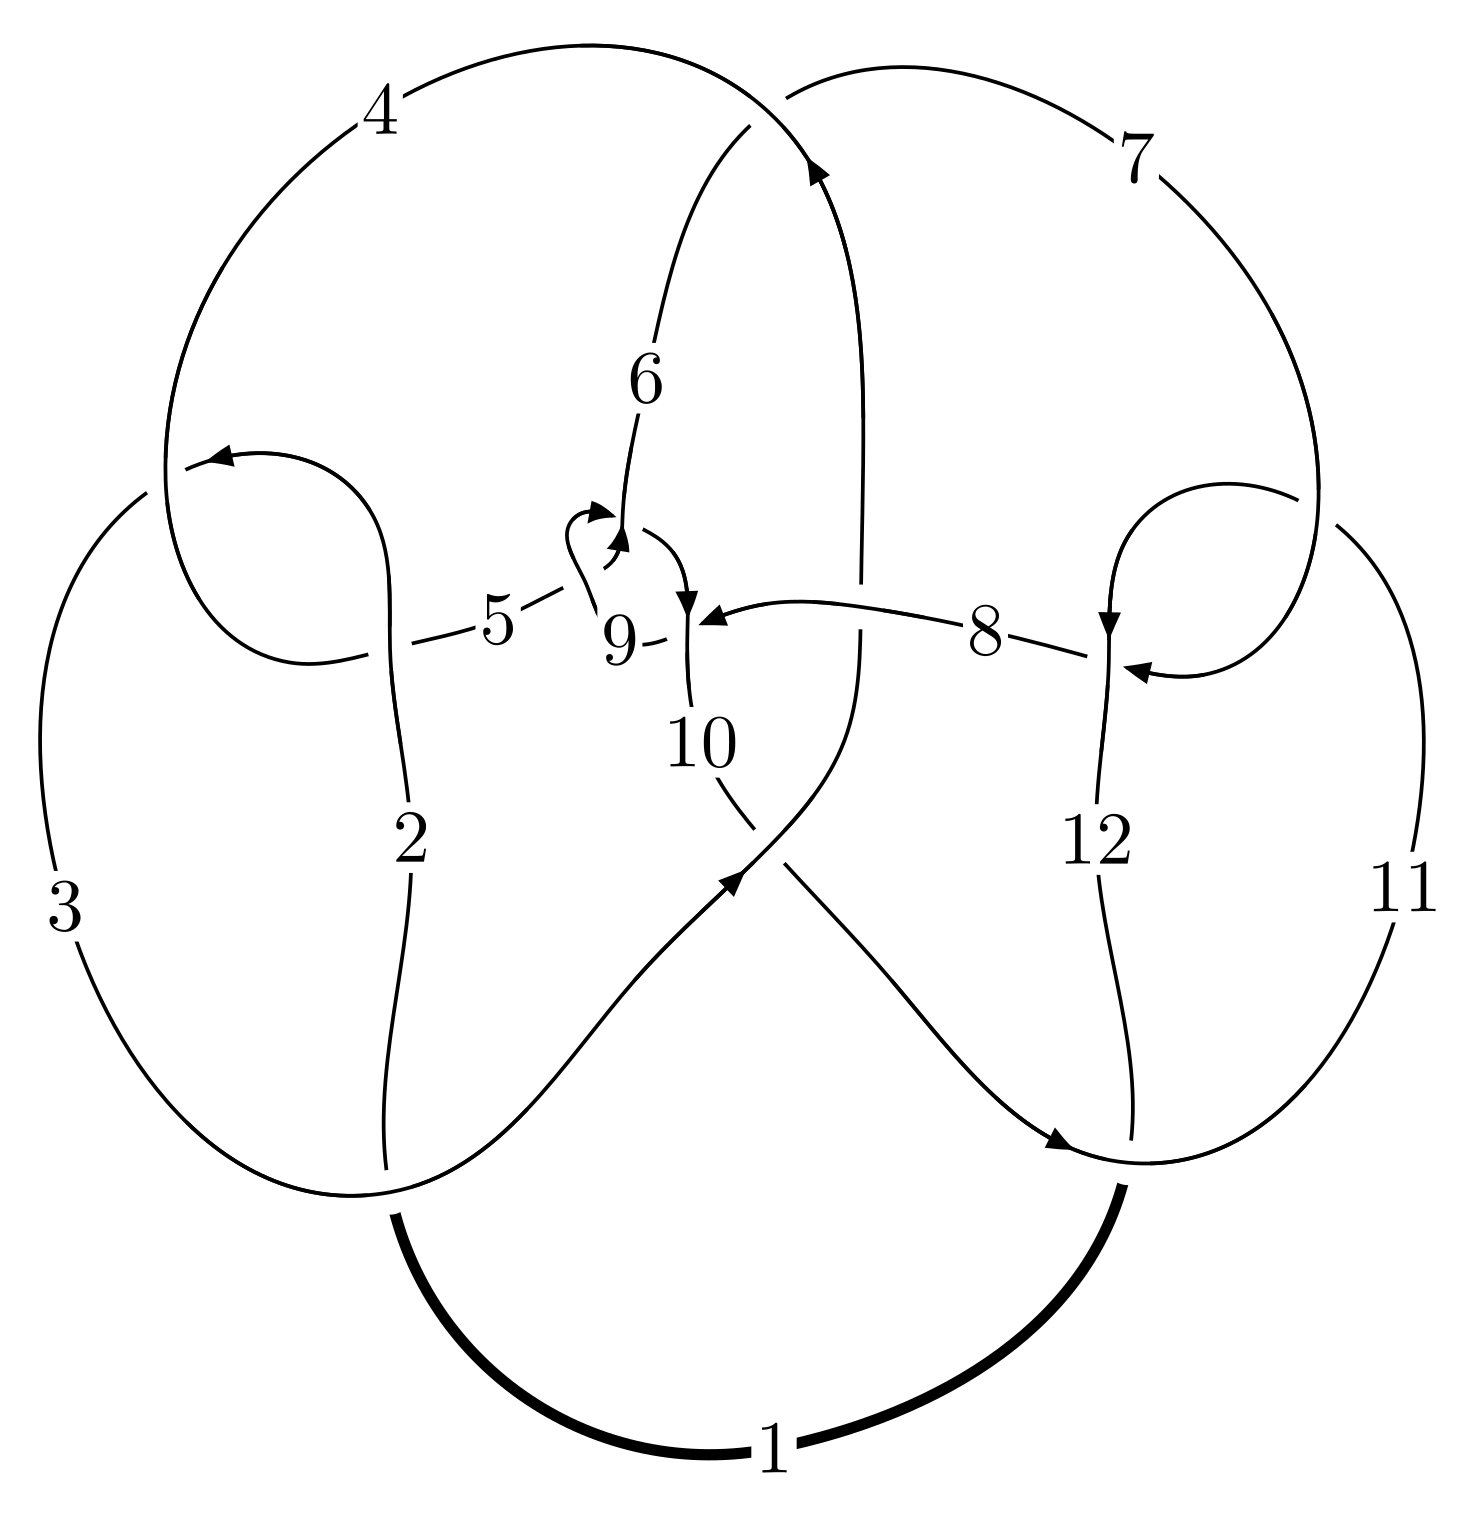
\includegraphics[width=112pt]{../../../GIT/diagram.site/Diagrams/png/2365_12n_0276.png}\\
\ \ \ A knot diagram\footnotemark}&
\allowdisplaybreaks
\textbf{Linearized knot diagam} \\
\cline{2-2}
 &
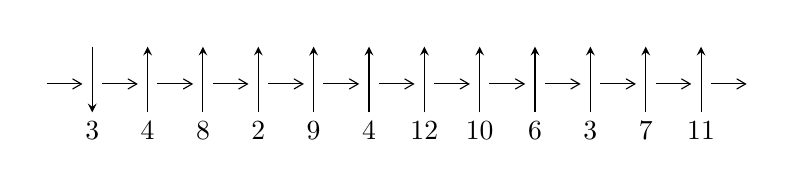
\begin{tikzpicture}[x=20pt, y=17pt]
	% nodes
	\node (C0) at (0, 0) {};
	\node (C1) at (1, 0) {};
	\node (C1U) at (1, +1) {};
	\node (C1D) at (1, -1) {3};

	\node (C2) at (2, 0) {};
	\node (C2U) at (2, +1) {};
	\node (C2D) at (2, -1) {4};

	\node (C3) at (3, 0) {};
	\node (C3U) at (3, +1) {};
	\node (C3D) at (3, -1) {8};

	\node (C4) at (4, 0) {};
	\node (C4U) at (4, +1) {};
	\node (C4D) at (4, -1) {2};

	\node (C5) at (5, 0) {};
	\node (C5U) at (5, +1) {};
	\node (C5D) at (5, -1) {9};

	\node (C6) at (6, 0) {};
	\node (C6U) at (6, +1) {};
	\node (C6D) at (6, -1) {4};

	\node (C7) at (7, 0) {};
	\node (C7U) at (7, +1) {};
	\node (C7D) at (7, -1) {12};

	\node (C8) at (8, 0) {};
	\node (C8U) at (8, +1) {};
	\node (C8D) at (8, -1) {10};

	\node (C9) at (9, 0) {};
	\node (C9U) at (9, +1) {};
	\node (C9D) at (9, -1) {6};

	\node (C10) at (10, 0) {};
	\node (C10U) at (10, +1) {};
	\node (C10D) at (10, -1) {3};

	\node (C11) at (11, 0) {};
	\node (C11U) at (11, +1) {};
	\node (C11D) at (11, -1) {7};

	\node (C12) at (12, 0) {};
	\node (C12U) at (12, +1) {};
	\node (C12D) at (12, -1) {11};
	\node (C13) at (13, 0) {};

	% arrows
	\draw[->,>={angle 60}]
	(C0) edge (C1) (C1) edge (C2) (C2) edge (C3) (C3) edge (C4) (C4) edge (C5) (C5) edge (C6) (C6) edge (C7) (C7) edge (C8) (C8) edge (C9) (C9) edge (C10) (C10) edge (C11) (C11) edge (C12) (C12) edge (C13) ;	\draw[->,>=stealth]
	(C1U) edge (C1D) (C2D) edge (C2U) (C3D) edge (C3U) (C4D) edge (C4U) (C5D) edge (C5U) (C6D) edge (C6U) (C7D) edge (C7U) (C8D) edge (C8U) (C9D) edge (C9U) (C10D) edge (C10U) (C11D) edge (C11U) (C12D) edge (C12U) ;
	\end{tikzpicture} \\
\hhline{~~} \\& 
\textbf{Solving Sequence} \\ \cline{2-2} 
 &
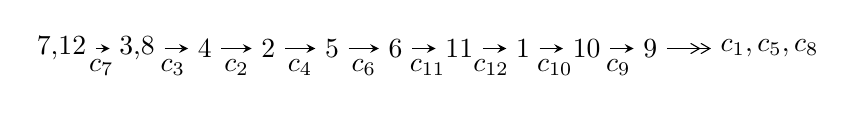
\begin{tikzpicture}[x=23pt, y=7pt]
	% node
	\node (A0) at (-1/8, 0) {7,12};
	\node (A1) at (17/16, 0) {3,8};
	\node (A2) at (17/8, 0) {4};
	\node (A3) at (25/8, 0) {2};
	\node (A4) at (33/8, 0) {5};
	\node (A5) at (41/8, 0) {6};
	\node (A6) at (49/8, 0) {11};
	\node (A7) at (57/8, 0) {1};
	\node (A8) at (65/8, 0) {10};
	\node (A9) at (73/8, 0) {9};
	\node (C1) at (1/2, -1) {$c_{7}$};
	\node (C2) at (13/8, -1) {$c_{3}$};
	\node (C3) at (21/8, -1) {$c_{2}$};
	\node (C4) at (29/8, -1) {$c_{4}$};
	\node (C5) at (37/8, -1) {$c_{6}$};
	\node (C6) at (45/8, -1) {$c_{11}$};
	\node (C7) at (53/8, -1) {$c_{12}$};
	\node (C8) at (61/8, -1) {$c_{10}$};
	\node (C9) at (69/8, -1) {$c_{9}$};
	\node (A10) at (11, 0) {$c_{1},c_{5},c_{8}$};

	% edge
	\draw[->,>=stealth]	
	(A0) edge (A1) (A1) edge (A2) (A2) edge (A3) (A3) edge (A4) (A4) edge (A5) (A5) edge (A6) (A6) edge (A7) (A7) edge (A8) (A8) edge (A9) ;
	\draw[->>,>={angle 60}]	
	(A9) edge (A10);
\end{tikzpicture} \\ 

\end{tabular} \\

\footnotetext{
The image of knot diagram is generated by the software ``\textbf{Draw programme}" developed by Andrew Bartholomew(\url{http://www.layer8.co.uk/maths/draw/index.htm\#Running-draw}), where we modified some parts for our purpose(\url{https://github.com/CATsTAILs/LinksPainter}).
}\phantom \\ \newline 
\centering \textbf{Ideals for irreducible components\footnotemark of $X_{\text{par}}$} 
 
\begin{align*}
I^u_{1}&=\langle 
- u^3- u^2+b+u+1,\;- u^2+a- u,\;u^4+2 u^3+u^2-2 u-1\rangle \\
I^u_{2}&=\langle 
u^3- u^2+b- u+1,\;-2 u^3+u^2+a+u,\;u^4- u^2+1\rangle \\
I^u_{3}&=\langle 
2 u^7-3 u^6+3 u^5+3 u^3+2 u^2+2 b-3 u-1,\;-3 u^7+4 u^6-3 u^5-3 u^4-3 u^3-3 u^2+2 a+4 u+3,\\
\phantom{I^u_{3}}&\phantom{= \langle  }u^8-2 u^7+2 u^6+u^4-2 u^2+1\rangle \\
I^u_{4}&=\langle 
2 u^7-3 u^6+3 u^5+3 u^3+2 u^2+2 b-3 u-1,\;- u^7+u^6-2 u^5+u^4-4 u^3- u^2+2 a- u,\\
\phantom{I^u_{4}}&\phantom{= \langle  }u^8-2 u^7+2 u^6+u^4-2 u^2+1\rangle \\
I^u_{5}&=\langle 
u^7+u^6+2 u^5+u^4+2 u^3+3 u^2+4 b+5 u+6,\;- u^7+3 u^6+2 u^5+3 u^4-10 u^3+5 u^2+8 a+11 u+10,\\
\phantom{I^u_{5}}&\phantom{= \langle  }u^8+3 u^7+4 u^6+u^5+7 u^3+15 u^2+12 u+4\rangle \\
I^u_{6}&=\langle 
u^3+b- u-1,\;- u^2+a+1,\;u^4- u^2+1\rangle \\
I^u_{7}&=\langle 
u^3+b- u-1,\;-2 u^3- u^2+a+u+1,\;u^4- u^2+1\rangle \\
I^u_{8}&=\langle 
u^3+u^2+b- u,\;a-1,\;u^4- u^2+1\rangle \\
\\
\end{align*}
\raggedright * 8 irreducible components of $\dim_{\mathbb{C}}=0$, with total 44 representations.\\
\footnotetext{All coefficients of polynomials are rational numbers. But the coefficients are sometimes approximated in decimal forms when there is not enough margin.}
\newpage
\renewcommand{\arraystretch}{1}
\centering \section*{I. $I^u_{1}= \langle - u^3- u^2+b+u+1,\;- u^2+a- u,\;u^4+2 u^3+u^2-2 u-1 \rangle$}
\flushleft \textbf{(i) Arc colorings}\\
\begin{tabular}{m{7pt} m{180pt} m{7pt} m{180pt} }
\flushright $a_{7}=$&$\begin{pmatrix}1\\0\end{pmatrix}$ \\
\flushright $a_{12}=$&$\begin{pmatrix}0\\u\end{pmatrix}$ \\
\flushright $a_{3}=$&$\begin{pmatrix}u^2+u\\u^3+u^2- u-1\end{pmatrix}$ \\
\flushright $a_{8}=$&$\begin{pmatrix}1\\- u^2\end{pmatrix}$ \\
\flushright $a_{4}=$&$\begin{pmatrix}u^2+2 u\\u^2- u-1\end{pmatrix}$ \\
\flushright $a_{2}=$&$\begin{pmatrix}2 u^2- u-1\\4 u^3+3 u^2-3 u-2\end{pmatrix}$ \\
\flushright $a_{5}=$&$\begin{pmatrix}5 u^3+4 u^2-2 u-2\\-3 u^3-10 u^2+5 u+4\end{pmatrix}$ \\
\flushright $a_{6}=$&$\begin{pmatrix}- u^3-4 u^2+2\\-4 u^3-2 u^2+4 u+2\end{pmatrix}$ \\
\flushright $a_{11}=$&$\begin{pmatrix}- u\\u\end{pmatrix}$ \\
\flushright $a_{1}=$&$\begin{pmatrix}u^3\\- u^3+u\end{pmatrix}$ \\
\flushright $a_{10}=$&$\begin{pmatrix}-2 u^3-3 u^2+1\\3 u^2-1\end{pmatrix}$ \\
\flushright $a_{9}=$&$\begin{pmatrix}-4 u^2+2\\-6 u^3-5 u^2+6 u+3\end{pmatrix}$\\&\end{tabular}
\flushleft \textbf{(ii) Obstruction class $= -1$}\\~\\
\flushleft \textbf{(iii) Cusp Shapes $= 6 u+16$}\\~\\
\newpage\renewcommand{\arraystretch}{1}
\flushleft \textbf{(iv) u-Polynomials at the component}\newline \\
\begin{tabular}{m{50pt}|m{274pt}}
Crossings & \hspace{64pt}u-Polynomials at each crossing \\
\hline $$\begin{aligned}c_{1}\end{aligned}$$&$\begin{aligned}
&u^4+10 u^3+27 u^2-22 u+1
\end{aligned}$\\
\hline $$\begin{aligned}c_{2},c_{4},c_{8}\\c_{12}\end{aligned}$$&$\begin{aligned}
&u^4-2 u^3+7 u^2-6 u+1
\end{aligned}$\\
\hline $$\begin{aligned}c_{3},c_{5},c_{7}\\c_{9},c_{11}\end{aligned}$$&$\begin{aligned}
&u^4-2 u^3+u^2+2 u-1
\end{aligned}$\\
\hline $$\begin{aligned}c_{6},c_{10}\end{aligned}$$&$\begin{aligned}
&u^4+10 u^2-16 u+4
\end{aligned}$\\
\hline
\end{tabular}\\~\\
\newpage\renewcommand{\arraystretch}{1}
\flushleft \textbf{(v) Riley Polynomials at the component}\newline \\
\begin{tabular}{m{50pt}|m{274pt}}
Crossings & \hspace{64pt}Riley Polynomials at each crossing \\
\hline $$\begin{aligned}c_{1}\end{aligned}$$&$\begin{aligned}
&y^4-46 y^3+1171 y^2-430 y+1
\end{aligned}$\\
\hline $$\begin{aligned}c_{2},c_{4},c_{8}\\c_{12}\end{aligned}$$&$\begin{aligned}
&y^4+10 y^3+27 y^2-22 y+1
\end{aligned}$\\
\hline $$\begin{aligned}c_{3},c_{5},c_{7}\\c_{9},c_{11}\end{aligned}$$&$\begin{aligned}
&y^4-2 y^3+7 y^2-6 y+1
\end{aligned}$\\
\hline $$\begin{aligned}c_{6},c_{10}\end{aligned}$$&$\begin{aligned}
&y^4+20 y^3+108 y^2-176 y+16
\end{aligned}$\\
\hline
\end{tabular}\\~\\
\newpage\flushleft \textbf{(vi) Complex Volumes and Cusp Shapes}
$$\begin{array}{c|c|c}  
\text{Solutions to }I^u_{1}& \I (\text{vol} + \sqrt{-1}CS) & \text{Cusp shape}\\
 \hline 
\begin{aligned}
u &= \phantom{-}0.883204\phantom{ +0.000000I} \\
a &= \phantom{-}1.66325\phantom{ +0.000000I} \\
b &= -0.414214\phantom{ +0.000000I}\end{aligned}
 & \phantom{-}4.18641\phantom{ +0.000000I} & \phantom{-}21.2990\phantom{ +0.000000I} \\ \hline\begin{aligned}
u &= -0.468990\phantom{ +0.000000I} \\
a &= -0.249038\phantom{ +0.000000I} \\
b &= -0.414214\phantom{ +0.000000I}\end{aligned}
 & \phantom{-}0.748389\phantom{ +0.000000I} & \phantom{-}13.1860\phantom{ +0.000000I} \\ \hline\begin{aligned}
u &= -1.20711 + 0.97832 I \\
a &= -0.70711 - 1.38355 I \\
b &= \phantom{-}2.41421\phantom{ +0.000000I}\end{aligned}
 & -17.2718 - 12.3509 I & \phantom{-}8.75736 + 5.86991 I \\ \hline\begin{aligned}
u &= -1.20711 - 0.97832 I \\
a &= -0.70711 + 1.38355 I \\
b &= \phantom{-}2.41421\phantom{ +0.000000I}\end{aligned}
 & -17.2718 + 12.3509 I & \phantom{-}8.75736 - 5.86991 I\\
 \hline 
 \end{array}$$\newpage\newpage\renewcommand{\arraystretch}{1}
\centering \section*{II. $I^u_{2}= \langle u^3- u^2+b- u+1,\;-2 u^3+u^2+a+u,\;u^4- u^2+1 \rangle$}
\flushleft \textbf{(i) Arc colorings}\\
\begin{tabular}{m{7pt} m{180pt} m{7pt} m{180pt} }
\flushright $a_{7}=$&$\begin{pmatrix}1\\0\end{pmatrix}$ \\
\flushright $a_{12}=$&$\begin{pmatrix}0\\u\end{pmatrix}$ \\
\flushright $a_{3}=$&$\begin{pmatrix}2 u^3- u^2- u\\- u^3+u^2+u-1\end{pmatrix}$ \\
\flushright $a_{8}=$&$\begin{pmatrix}1\\- u^2\end{pmatrix}$ \\
\flushright $a_{4}=$&$\begin{pmatrix}2 u^3- u^2-2 u\\u^2+u-1\end{pmatrix}$ \\
\flushright $a_{2}=$&$\begin{pmatrix}2 u^3+u-1\\-2 u^3+u^2+u\end{pmatrix}$ \\
\flushright $a_{5}=$&$\begin{pmatrix}- u^3\\u^3- u\end{pmatrix}$ \\
\flushright $a_{6}=$&$\begin{pmatrix}-3 u^3\\2 u^3-2 u\end{pmatrix}$ \\
\flushright $a_{11}=$&$\begin{pmatrix}- u\\u\end{pmatrix}$ \\
\flushright $a_{1}=$&$\begin{pmatrix}u^3\\- u^3+u\end{pmatrix}$ \\
\flushright $a_{10}=$&$\begin{pmatrix}u^2-3\\u^2+1\end{pmatrix}$ \\
\flushright $a_{9}=$&$\begin{pmatrix}-2 u^2\\u^2-1\end{pmatrix}$\\&\end{tabular}
\flushleft \textbf{(ii) Obstruction class $= 1$}\\~\\
\flushleft \textbf{(iii) Cusp Shapes $= -12 u^2+16$}\\~\\
\newpage\renewcommand{\arraystretch}{1}
\flushleft \textbf{(iv) u-Polynomials at the component}\newline \\
\begin{tabular}{m{50pt}|m{274pt}}
Crossings & \hspace{64pt}u-Polynomials at each crossing \\
\hline $$\begin{aligned}c_{1},c_{4},c_{12}\end{aligned}$$&$\begin{aligned}
&(u^2- u+1)^2
\end{aligned}$\\
\hline $$\begin{aligned}c_{2},c_{8}\end{aligned}$$&$\begin{aligned}
&(u^2+u+1)^2
\end{aligned}$\\
\hline $$\begin{aligned}c_{3},c_{5},c_{7}\\c_{9},c_{11}\end{aligned}$$&$\begin{aligned}
&u^4- u^2+1
\end{aligned}$\\
\hline $$\begin{aligned}c_{6}\end{aligned}$$&$\begin{aligned}
&u^4+2 u^3+2 u^2+4 u+4
\end{aligned}$\\
\hline $$\begin{aligned}c_{10}\end{aligned}$$&$\begin{aligned}
&u^4-2 u^3+2 u^2-4 u+4
\end{aligned}$\\
\hline
\end{tabular}\\~\\
\newpage\renewcommand{\arraystretch}{1}
\flushleft \textbf{(v) Riley Polynomials at the component}\newline \\
\begin{tabular}{m{50pt}|m{274pt}}
Crossings & \hspace{64pt}Riley Polynomials at each crossing \\
\hline $$\begin{aligned}c_{1},c_{2},c_{4}\\c_{8},c_{12}\end{aligned}$$&$\begin{aligned}
&(y^2+y+1)^2
\end{aligned}$\\
\hline $$\begin{aligned}c_{3},c_{5},c_{7}\\c_{9},c_{11}\end{aligned}$$&$\begin{aligned}
&(y^2- y+1)^2
\end{aligned}$\\
\hline $$\begin{aligned}c_{6},c_{10}\end{aligned}$$&$\begin{aligned}
&y^4-4 y^2+16
\end{aligned}$\\
\hline
\end{tabular}\\~\\
\newpage\flushleft \textbf{(vi) Complex Volumes and Cusp Shapes}
$$\begin{array}{c|c|c}  
\text{Solutions to }I^u_{2}& \I (\text{vol} + \sqrt{-1}CS) & \text{Cusp shape}\\
 \hline 
\begin{aligned}
u &= \phantom{-}0.866025 + 0.500000 I \\
a &= -1.36603 + 0.63397 I \\
b &= \phantom{-}0.366025 + 0.366025 I\end{aligned}
 & \phantom{-0.000000 -}6.08965 I & \phantom{-}10.0000 - 10.3923 I \\ \hline\begin{aligned}
u &= \phantom{-}0.866025 - 0.500000 I \\
a &= -1.36603 - 0.63397 I \\
b &= \phantom{-}0.366025 - 0.366025 I\end{aligned}
 & \phantom{-0.000000 } -6.08965 I & \phantom{-}10.0000 + 10.3923 I \\ \hline\begin{aligned}
u &= -0.866025 + 0.500000 I \\
a &= \phantom{-}0.36603 + 2.36603 I \\
b &= -1.36603 - 1.36603 I\end{aligned}
 & \phantom{-0.000000 } -6.08965 I & \phantom{-}10.0000 + 10.3923 I \\ \hline\begin{aligned}
u &= -0.866025 - 0.500000 I \\
a &= \phantom{-}0.36603 - 2.36603 I \\
b &= -1.36603 + 1.36603 I\end{aligned}
 & \phantom{-0.000000 -}6.08965 I & \phantom{-}10.0000 - 10.3923 I\\
 \hline 
 \end{array}$$\newpage\newpage\renewcommand{\arraystretch}{1}
\centering \section*{III. $I^u_{3}= \langle 2 u^7-3 u^6+3 u^5+3 u^3+2 u^2+2 b-3 u-1,\;-3 u^7+4 u^6+\cdots+2 a+3,\;u^8-2 u^7+2 u^6+u^4-2 u^2+1 \rangle$}
\flushleft \textbf{(i) Arc colorings}\\
\begin{tabular}{m{7pt} m{180pt} m{7pt} m{180pt} }
\flushright $a_{7}=$&$\begin{pmatrix}1\\0\end{pmatrix}$ \\
\flushright $a_{12}=$&$\begin{pmatrix}0\\u\end{pmatrix}$ \\
\flushright $a_{3}=$&$\begin{pmatrix}\frac{3}{2} u^7-2 u^6+\cdots-2 u-\frac{3}{2}\\- u^7+\frac{3}{2} u^6+\cdots+\frac{3}{2} u+\frac{1}{2}\end{pmatrix}$ \\
\flushright $a_{8}=$&$\begin{pmatrix}1\\- u^2\end{pmatrix}$ \\
\flushright $a_{4}=$&$\begin{pmatrix}u^7- u^6+2 u^4+u^3+u^2-2 u-2\\-\frac{1}{2} u^7+u^6+\cdots+u+\frac{1}{2}\end{pmatrix}$ \\
\flushright $a_{2}=$&$\begin{pmatrix}2 u^7-\frac{5}{2} u^6+\cdots-\frac{1}{2} u-\frac{3}{2}\\- u^7+\frac{1}{2} u^6+\cdots+\frac{3}{2} u+\frac{1}{2}\end{pmatrix}$ \\
\flushright $a_{5}=$&$\begin{pmatrix}-2 u^7+3 u^6-2 u^5-2 u^4-3 u^3+2 u+1\\2 u^5- u^4+u^3+u^2- u-1\end{pmatrix}$ \\
\flushright $a_{6}=$&$\begin{pmatrix}\frac{3}{2} u^7-2 u^6+\cdots-2 u-\frac{1}{2}\\-\frac{1}{2} u^7+\frac{1}{2} u^6+\cdots+\frac{1}{2} u+1\end{pmatrix}$ \\
\flushright $a_{11}=$&$\begin{pmatrix}- u\\u\end{pmatrix}$ \\
\flushright $a_{1}=$&$\begin{pmatrix}u^3\\- u^3+u\end{pmatrix}$ \\
\flushright $a_{10}=$&$\begin{pmatrix}\frac{3}{2} u^7-2 u^6+\cdots-2 u-\frac{3}{2}\\-\frac{1}{2} u^7+\frac{1}{2} u^6+\cdots+\frac{3}{2} u+1\end{pmatrix}$ \\
\flushright $a_{9}=$&$\begin{pmatrix}\frac{1}{2} u^7-\frac{1}{2} u^6+\cdots+\frac{1}{2} u^2-\frac{3}{2} u\\\frac{1}{2} u^6-\frac{1}{2} u^5+\cdots+\frac{1}{2} u+\frac{1}{2}\end{pmatrix}$\\&\end{tabular}
\flushleft \textbf{(ii) Obstruction class $= -1$}\\~\\
\flushleft \textbf{(iii) Cusp Shapes $= -4 u^7+4 u^6-2 u^5-4 u^4-8 u^3-4 u^2+6 u+16$}\\~\\
\newpage\renewcommand{\arraystretch}{1}
\flushleft \textbf{(iv) u-Polynomials at the component}\newline \\
\begin{tabular}{m{50pt}|m{274pt}}
Crossings & \hspace{64pt}u-Polynomials at each crossing \\
\hline $$\begin{aligned}c_{1}\end{aligned}$$&$\begin{aligned}
&u^8+19 u^7+\cdots+1248 u+256
\end{aligned}$\\
\hline $$\begin{aligned}c_{2},c_{4}\end{aligned}$$&$\begin{aligned}
&u^8- u^7+10 u^6-13 u^5+42 u^4-41 u^3+57 u^2-24 u+16
\end{aligned}$\\
\hline $$\begin{aligned}c_{3}\end{aligned}$$&$\begin{aligned}
&u^8-3 u^7+4 u^6- u^5-7 u^3+15 u^2-12 u+4
\end{aligned}$\\
\hline $$\begin{aligned}c_{5},c_{7},c_{9}\\c_{11}\end{aligned}$$&$\begin{aligned}
&u^8+2 u^7+2 u^6+u^4-2 u^2+1
\end{aligned}$\\
\hline $$\begin{aligned}c_{6},c_{10}\end{aligned}$$&$\begin{aligned}
&u^8+7 u^7+25 u^6+52 u^5+54 u^4+16 u^3-8 u^2+4
\end{aligned}$\\
\hline $$\begin{aligned}c_{8},c_{12}\end{aligned}$$&$\begin{aligned}
&u^8+6 u^6-5 u^4+6 u^2-4 u+1
\end{aligned}$\\
\hline
\end{tabular}\\~\\
\newpage\renewcommand{\arraystretch}{1}
\flushleft \textbf{(v) Riley Polynomials at the component}\newline \\
\begin{tabular}{m{50pt}|m{274pt}}
Crossings & \hspace{64pt}Riley Polynomials at each crossing \\
\hline $$\begin{aligned}c_{1}\end{aligned}$$&$\begin{aligned}
&y^8-45 y^7+\cdots-213504 y+65536
\end{aligned}$\\
\hline $$\begin{aligned}c_{2},c_{4}\end{aligned}$$&$\begin{aligned}
&y^8+19 y^7+\cdots+1248 y+256
\end{aligned}$\\
\hline $$\begin{aligned}c_{3}\end{aligned}$$&$\begin{aligned}
&y^8- y^7+10 y^6-13 y^5+42 y^4-41 y^3+57 y^2-24 y+16
\end{aligned}$\\
\hline $$\begin{aligned}c_{5},c_{7},c_{9}\\c_{11}\end{aligned}$$&$\begin{aligned}
&y^8+6 y^6-5 y^4+6 y^2-4 y+1
\end{aligned}$\\
\hline $$\begin{aligned}c_{6},c_{10}\end{aligned}$$&$\begin{aligned}
&y^8+y^7+5 y^6-244 y^5+860 y^4-920 y^3+496 y^2-64 y+16
\end{aligned}$\\
\hline $$\begin{aligned}c_{8},c_{12}\end{aligned}$$&$\begin{aligned}
&y^8+12 y^7+26 y^6-48 y^5+99 y^4-48 y^3+26 y^2-4 y+1
\end{aligned}$\\
\hline
\end{tabular}\\~\\
\newpage\flushleft \textbf{(vi) Complex Volumes and Cusp Shapes}
$$\begin{array}{c|c|c}  
\text{Solutions to }I^u_{3}& \I (\text{vol} + \sqrt{-1}CS) & \text{Cusp shape}\\
 \hline 
\begin{aligned}
u &= -0.273242 + 1.017440 I \\
a &= -0.038323 + 1.295230 I \\
b &= \phantom{-}0.307345 + 0.392902 I\end{aligned}
 & -3.00645 - 3.35673 I & \phantom{-}6.09240 + 3.01308 I \\ \hline\begin{aligned}
u &= -0.273242 - 1.017440 I \\
a &= -0.038323 - 1.295230 I \\
b &= \phantom{-}0.307345 - 0.392902 I\end{aligned}
 & -3.00645 + 3.35673 I & \phantom{-}6.09240 - 3.01308 I \\ \hline\begin{aligned}
u &= \phantom{-}0.796321 + 0.241667 I \\
a &= -1.41328 + 1.73710 I \\
b &= \phantom{-}0.545221 - 1.041750 I\end{aligned}
 & \phantom{-}1.17763 + 4.62470 I & \phantom{-}15.0023 - 5.8935 I \\ \hline\begin{aligned}
u &= \phantom{-}0.796321 - 0.241667 I \\
a &= -1.41328 - 1.73710 I \\
b &= \phantom{-}0.545221 + 1.041750 I\end{aligned}
 & \phantom{-}1.17763 - 4.62470 I & \phantom{-}15.0023 + 5.8935 I \\ \hline\begin{aligned}
u &= -0.666028 + 0.230992 I \\
a &= \phantom{-}0.439021 - 0.264857 I \\
b &= -0.768780 - 0.277812 I\end{aligned}
 & \phantom{-}0.403528 - 0.080080 I & \phantom{-}11.24335 + 0.17507 I \\ \hline\begin{aligned}
u &= -0.666028 - 0.230992 I \\
a &= \phantom{-}0.439021 + 0.264857 I \\
b &= -0.768780 + 0.277812 I\end{aligned}
 & \phantom{-}0.403528 + 0.080080 I & \phantom{-}11.24335 - 0.17507 I \\ \hline\begin{aligned}
u &= \phantom{-}1.14295 + 1.14532 I \\
a &= \phantom{-}0.512578 - 0.434756 I \\
b &= -2.08379 - 0.09016 I\end{aligned}
 & -18.3139 + 4.2344 I & \phantom{-}7.66195 - 1.86062 I \\ \hline\begin{aligned}
u &= \phantom{-}1.14295 - 1.14532 I \\
a &= \phantom{-}0.512578 + 0.434756 I \\
b &= -2.08379 + 0.09016 I\end{aligned}
 & -18.3139 - 4.2344 I & \phantom{-}7.66195 + 1.86062 I\\
 \hline 
 \end{array}$$\newpage\newpage\renewcommand{\arraystretch}{1}
\centering \section*{IV. $I^u_{4}= \langle 2 u^7-3 u^6+3 u^5+3 u^3+2 u^2+2 b-3 u-1,\;- u^7+u^6-2 u^5+u^4-4 u^3- u^2+2 a- u,\;u^8-2 u^7+2 u^6+u^4-2 u^2+1 \rangle$}
\flushleft \textbf{(i) Arc colorings}\\
\begin{tabular}{m{7pt} m{180pt} m{7pt} m{180pt} }
\flushright $a_{7}=$&$\begin{pmatrix}1\\0\end{pmatrix}$ \\
\flushright $a_{12}=$&$\begin{pmatrix}0\\u\end{pmatrix}$ \\
\flushright $a_{3}=$&$\begin{pmatrix}\frac{1}{2} u^7-\frac{1}{2} u^6+\cdots+\frac{1}{2} u^2+\frac{1}{2} u\\- u^7+\frac{3}{2} u^6+\cdots+\frac{3}{2} u+\frac{1}{2}\end{pmatrix}$ \\
\flushright $a_{8}=$&$\begin{pmatrix}1\\- u^2\end{pmatrix}$ \\
\flushright $a_{4}=$&$\begin{pmatrix}\frac{1}{2} u^7-\frac{1}{2} u^6+\cdots+\frac{1}{2} u^2+\frac{3}{2} u\\- u^7+\frac{3}{2} u^6+\cdots+\frac{3}{2} u+\frac{1}{2}\end{pmatrix}$ \\
\flushright $a_{2}=$&$\begin{pmatrix}-\frac{1}{2} u^7+u^6+\cdots+u+\frac{1}{2}\\-\frac{1}{2} u^7+\frac{1}{2} u^6+\cdots-\frac{1}{2} u^2+\frac{1}{2} u\end{pmatrix}$ \\
\flushright $a_{5}=$&$\begin{pmatrix}u^5+2 u^3+u\\- u^7- u^5-2 u^3+u\end{pmatrix}$ \\
\flushright $a_{6}=$&$\begin{pmatrix}-2 u^7+\frac{5}{2} u^6+\cdots+\frac{5}{2} u+\frac{9}{2}\\-\frac{1}{2} u^6+\frac{3}{2} u^5+\cdots-\frac{3}{2} u-\frac{1}{2}\end{pmatrix}$ \\
\flushright $a_{11}=$&$\begin{pmatrix}- u\\u\end{pmatrix}$ \\
\flushright $a_{1}=$&$\begin{pmatrix}u^3\\- u^3+u\end{pmatrix}$ \\
\flushright $a_{10}=$&$\begin{pmatrix}-\frac{3}{2} u^7+2 u^6+\cdots-\frac{3}{2} u^2+\frac{1}{2}\\u^7- u^6+u^5+u^4+u^3+u^2- u-1\end{pmatrix}$ \\
\flushright $a_{9}=$&$\begin{pmatrix}-\frac{5}{2} u^7+3 u^6+\cdots+3 u+\frac{9}{2}\\-\frac{1}{2} u^6+\frac{1}{2} u^5+\cdots-\frac{3}{2} u-\frac{1}{2}\end{pmatrix}$\\&\end{tabular}
\flushleft \textbf{(ii) Obstruction class $= -1$}\\~\\
\flushleft \textbf{(iii) Cusp Shapes $= -4 u^7+4 u^6-2 u^5-4 u^4-8 u^3-4 u^2+6 u+16$}\\~\\
\newpage\renewcommand{\arraystretch}{1}
\flushleft \textbf{(iv) u-Polynomials at the component}\newline \\
\begin{tabular}{m{50pt}|m{274pt}}
Crossings & \hspace{64pt}u-Polynomials at each crossing \\
\hline $$\begin{aligned}c_{1}\end{aligned}$$&$\begin{aligned}
&u^8+12 u^7+26 u^6-48 u^5+99 u^4-48 u^3+26 u^2-4 u+1
\end{aligned}$\\
\hline $$\begin{aligned}c_{2},c_{4},c_{12}\end{aligned}$$&$\begin{aligned}
&u^8+6 u^6-5 u^4+6 u^2-4 u+1
\end{aligned}$\\
\hline $$\begin{aligned}c_{3},c_{7},c_{11}\end{aligned}$$&$\begin{aligned}
&u^8+2 u^7+2 u^6+u^4-2 u^2+1
\end{aligned}$\\
\hline $$\begin{aligned}c_{5},c_{9}\end{aligned}$$&$\begin{aligned}
&u^8-3 u^7+4 u^6- u^5-7 u^3+15 u^2-12 u+4
\end{aligned}$\\
\hline $$\begin{aligned}c_{6}\end{aligned}$$&$\begin{aligned}
&u^8+12 u^6-16 u^5+49 u^4-56 u^3+78 u^2-54 u+27
\end{aligned}$\\
\hline $$\begin{aligned}c_{8}\end{aligned}$$&$\begin{aligned}
&u^8- u^7+10 u^6-13 u^5+42 u^4-41 u^3+57 u^2-24 u+16
\end{aligned}$\\
\hline $$\begin{aligned}c_{10}\end{aligned}$$&$\begin{aligned}
&u^8-4 u^7+18 u^6-58 u^5+111 u^4-126 u^3+92 u^2-40 u+11
\end{aligned}$\\
\hline
\end{tabular}\\~\\
\newpage\renewcommand{\arraystretch}{1}
\flushleft \textbf{(v) Riley Polynomials at the component}\newline \\
\begin{tabular}{m{50pt}|m{274pt}}
Crossings & \hspace{64pt}Riley Polynomials at each crossing \\
\hline $$\begin{aligned}c_{1}\end{aligned}$$&$\begin{aligned}
&y^8-92 y^7+\cdots+36 y+1
\end{aligned}$\\
\hline $$\begin{aligned}c_{2},c_{4},c_{12}\end{aligned}$$&$\begin{aligned}
&y^8+12 y^7+26 y^6-48 y^5+99 y^4-48 y^3+26 y^2-4 y+1
\end{aligned}$\\
\hline $$\begin{aligned}c_{3},c_{7},c_{11}\end{aligned}$$&$\begin{aligned}
&y^8+6 y^6-5 y^4+6 y^2-4 y+1
\end{aligned}$\\
\hline $$\begin{aligned}c_{5},c_{9}\end{aligned}$$&$\begin{aligned}
&y^8- y^7+10 y^6-13 y^5+42 y^4-41 y^3+57 y^2-24 y+16
\end{aligned}$\\
\hline $$\begin{aligned}c_{6}\end{aligned}$$&$\begin{aligned}
&y^8+24 y^7+\cdots+1296 y+729
\end{aligned}$\\
\hline $$\begin{aligned}c_{8}\end{aligned}$$&$\begin{aligned}
&y^8+19 y^7+\cdots+1248 y+256
\end{aligned}$\\
\hline $$\begin{aligned}c_{10}\end{aligned}$$&$\begin{aligned}
&y^8+20 y^7+82 y^6-192 y^5+719 y^4+304 y^3+826 y^2+424 y+121
\end{aligned}$\\
\hline
\end{tabular}\\~\\
\newpage\flushleft \textbf{(vi) Complex Volumes and Cusp Shapes}
$$\begin{array}{c|c|c}  
\text{Solutions to }I^u_{4}& \I (\text{vol} + \sqrt{-1}CS) & \text{Cusp shape}\\
 \hline 
\begin{aligned}
u &= -0.273242 + 1.017440 I \\
a &= \phantom{-}0.170826 - 0.749091 I \\
b &= \phantom{-}0.307345 + 0.392902 I\end{aligned}
 & -3.00645 - 3.35673 I & \phantom{-}6.09240 + 3.01308 I \\ \hline\begin{aligned}
u &= -0.273242 - 1.017440 I \\
a &= \phantom{-}0.170826 + 0.749091 I \\
b &= \phantom{-}0.307345 - 0.392902 I\end{aligned}
 & -3.00645 + 3.35673 I & \phantom{-}6.09240 - 3.01308 I \\ \hline\begin{aligned}
u &= \phantom{-}0.796321 + 0.241667 I \\
a &= \phantom{-}1.33140 + 1.33913 I \\
b &= \phantom{-}0.545221 - 1.041750 I\end{aligned}
 & \phantom{-}1.17763 + 4.62470 I & \phantom{-}15.0023 - 5.8935 I \\ \hline\begin{aligned}
u &= \phantom{-}0.796321 - 0.241667 I \\
a &= \phantom{-}1.33140 - 1.33913 I \\
b &= \phantom{-}0.545221 + 1.041750 I\end{aligned}
 & \phantom{-}1.17763 - 4.62470 I & \phantom{-}15.0023 + 5.8935 I \\ \hline\begin{aligned}
u &= -0.666028 + 0.230992 I \\
a &= -0.471568 + 0.932013 I \\
b &= -0.768780 - 0.277812 I\end{aligned}
 & \phantom{-}0.403528 - 0.080080 I & \phantom{-}11.24335 + 0.17507 I \\ \hline\begin{aligned}
u &= -0.666028 - 0.230992 I \\
a &= -0.471568 - 0.932013 I \\
b &= -0.768780 + 0.277812 I\end{aligned}
 & \phantom{-}0.403528 + 0.080080 I & \phantom{-}11.24335 - 0.17507 I \\ \hline\begin{aligned}
u &= \phantom{-}1.14295 + 1.14532 I \\
a &= \phantom{-}0.469343 - 1.233450 I \\
b &= -2.08379 - 0.09016 I\end{aligned}
 & -18.3139 + 4.2344 I & \phantom{-}7.66195 - 1.86062 I \\ \hline\begin{aligned}
u &= \phantom{-}1.14295 - 1.14532 I \\
a &= \phantom{-}0.469343 + 1.233450 I \\
b &= -2.08379 + 0.09016 I\end{aligned}
 & -18.3139 - 4.2344 I & \phantom{-}7.66195 + 1.86062 I\\
 \hline 
 \end{array}$$\newpage\newpage\renewcommand{\arraystretch}{1}
\centering \section*{V. $I^u_{5}= \langle u^7+u^6+2 u^5+u^4+2 u^3+3 u^2+4 b+5 u+6,\;- u^7+3 u^6+\cdots+8 a+10,\;u^8+3 u^7+4 u^6+u^5+7 u^3+15 u^2+12 u+4 \rangle$}
\flushleft \textbf{(i) Arc colorings}\\
\begin{tabular}{m{7pt} m{180pt} m{7pt} m{180pt} }
\flushright $a_{7}=$&$\begin{pmatrix}1\\0\end{pmatrix}$ \\
\flushright $a_{12}=$&$\begin{pmatrix}0\\u\end{pmatrix}$ \\
\flushright $a_{3}=$&$\begin{pmatrix}\frac{1}{8} u^7-\frac{3}{8} u^6+\cdots-\frac{11}{8} u-\frac{5}{4}\\-\frac{1}{4} u^7-\frac{1}{4} u^6+\cdots-\frac{5}{4} u-\frac{3}{2}\end{pmatrix}$ \\
\flushright $a_{8}=$&$\begin{pmatrix}1\\- u^2\end{pmatrix}$ \\
\flushright $a_{4}=$&$\begin{pmatrix}\frac{11}{8} u^7+\frac{15}{8} u^6+\cdots+\frac{47}{8} u+\frac{1}{4}\\-\frac{5}{4} u^7-\frac{13}{4} u^6+\cdots-\frac{57}{4} u-\frac{15}{2}\end{pmatrix}$ \\
\flushright $a_{2}=$&$\begin{pmatrix}-\frac{9}{8} u^7-\frac{17}{8} u^6+\cdots-\frac{57}{8} u-\frac{9}{4}\\\frac{5}{4} u^7+\frac{17}{4} u^6+\cdots+\frac{65}{4} u+\frac{13}{2}\end{pmatrix}$ \\
\flushright $a_{5}=$&$\begin{pmatrix}u^7+u^6+u^5- u^4+2 u^3+5 u^2+4 u\\-3 u^7-6 u^6-3 u^5+2 u^4-4 u^3-18 u^2-19 u-8\end{pmatrix}$ \\
\flushright $a_{6}=$&$\begin{pmatrix}-\frac{17}{8} u^7-\frac{25}{8} u^6+\cdots-\frac{81}{8} u-\frac{1}{4}\\\frac{11}{4} u^7+\frac{23}{4} u^6+\cdots+\frac{99}{4} u+\frac{23}{2}\end{pmatrix}$ \\
\flushright $a_{11}=$&$\begin{pmatrix}- u\\u\end{pmatrix}$ \\
\flushright $a_{1}=$&$\begin{pmatrix}u^3\\- u^3+u\end{pmatrix}$ \\
\flushright $a_{10}=$&$\begin{pmatrix}-2.37500 u^{7}-5.37500 u^{6}+\cdots-21.3750 u-8.75000\\-\frac{1}{4} u^7+\frac{3}{4} u^6+\cdots+\frac{19}{4} u+\frac{7}{2}\end{pmatrix}$ \\
\flushright $a_{9}=$&$\begin{pmatrix}-\frac{11}{8} u^7-\frac{23}{8} u^6+\cdots-\frac{87}{8} u-\frac{13}{4}\\\frac{1}{4} u^7+\frac{9}{4} u^6+\cdots+\frac{29}{4} u+\frac{7}{2}\end{pmatrix}$\\&\end{tabular}
\flushleft \textbf{(ii) Obstruction class $= -1$}\\~\\
\flushleft \textbf{(iii) Cusp Shapes $= -4 u^6-4 u^5-2 u^4+6 u^3-10 u^2-20 u-2$}\\~\\
\newpage\renewcommand{\arraystretch}{1}
\flushleft \textbf{(iv) u-Polynomials at the component}\newline \\
\begin{tabular}{m{50pt}|m{274pt}}
Crossings & \hspace{64pt}u-Polynomials at each crossing \\
\hline $$\begin{aligned}c_{1}\end{aligned}$$&$\begin{aligned}
&u^8+12 u^7+26 u^6-48 u^5+99 u^4-48 u^3+26 u^2-4 u+1
\end{aligned}$\\
\hline $$\begin{aligned}c_{2},c_{4},c_{8}\end{aligned}$$&$\begin{aligned}
&u^8+6 u^6-5 u^4+6 u^2-4 u+1
\end{aligned}$\\
\hline $$\begin{aligned}c_{3},c_{5},c_{9}\end{aligned}$$&$\begin{aligned}
&u^8+2 u^7+2 u^6+u^4-2 u^2+1
\end{aligned}$\\
\hline $$\begin{aligned}c_{6}\end{aligned}$$&$\begin{aligned}
&u^8-4 u^7+18 u^6-58 u^5+111 u^4-126 u^3+92 u^2-40 u+11
\end{aligned}$\\
\hline $$\begin{aligned}c_{7},c_{11}\end{aligned}$$&$\begin{aligned}
&u^8-3 u^7+4 u^6- u^5-7 u^3+15 u^2-12 u+4
\end{aligned}$\\
\hline $$\begin{aligned}c_{10}\end{aligned}$$&$\begin{aligned}
&u^8+12 u^6-16 u^5+49 u^4-56 u^3+78 u^2-54 u+27
\end{aligned}$\\
\hline $$\begin{aligned}c_{12}\end{aligned}$$&$\begin{aligned}
&u^8- u^7+10 u^6-13 u^5+42 u^4-41 u^3+57 u^2-24 u+16
\end{aligned}$\\
\hline
\end{tabular}\\~\\
\newpage\renewcommand{\arraystretch}{1}
\flushleft \textbf{(v) Riley Polynomials at the component}\newline \\
\begin{tabular}{m{50pt}|m{274pt}}
Crossings & \hspace{64pt}Riley Polynomials at each crossing \\
\hline $$\begin{aligned}c_{1}\end{aligned}$$&$\begin{aligned}
&y^8-92 y^7+\cdots+36 y+1
\end{aligned}$\\
\hline $$\begin{aligned}c_{2},c_{4},c_{8}\end{aligned}$$&$\begin{aligned}
&y^8+12 y^7+26 y^6-48 y^5+99 y^4-48 y^3+26 y^2-4 y+1
\end{aligned}$\\
\hline $$\begin{aligned}c_{3},c_{5},c_{9}\end{aligned}$$&$\begin{aligned}
&y^8+6 y^6-5 y^4+6 y^2-4 y+1
\end{aligned}$\\
\hline $$\begin{aligned}c_{6}\end{aligned}$$&$\begin{aligned}
&y^8+20 y^7+82 y^6-192 y^5+719 y^4+304 y^3+826 y^2+424 y+121
\end{aligned}$\\
\hline $$\begin{aligned}c_{7},c_{11}\end{aligned}$$&$\begin{aligned}
&y^8- y^7+10 y^6-13 y^5+42 y^4-41 y^3+57 y^2-24 y+16
\end{aligned}$\\
\hline $$\begin{aligned}c_{10}\end{aligned}$$&$\begin{aligned}
&y^8+24 y^7+\cdots+1296 y+729
\end{aligned}$\\
\hline $$\begin{aligned}c_{12}\end{aligned}$$&$\begin{aligned}
&y^8+19 y^7+\cdots+1248 y+256
\end{aligned}$\\
\hline
\end{tabular}\\~\\
\newpage\flushleft \textbf{(vi) Complex Volumes and Cusp Shapes}
$$\begin{array}{c|c|c}  
\text{Solutions to }I^u_{5}& \I (\text{vol} + \sqrt{-1}CS) & \text{Cusp shape}\\
 \hline 
\begin{aligned}
u &= -0.937027 + 0.585611 I \\
a &= \phantom{-}0.68623 + 1.54063 I \\
b &= -1.261650 - 0.312913 I\end{aligned}
 & \phantom{-}1.17763 - 4.62470 I & \phantom{-}15.0023 + 5.8935 I \\ \hline\begin{aligned}
u &= -0.937027 - 0.585611 I \\
a &= \phantom{-}0.68623 - 1.54063 I \\
b &= -1.261650 + 0.312913 I\end{aligned}
 & \phantom{-}1.17763 + 4.62470 I & \phantom{-}15.0023 - 5.8935 I \\ \hline\begin{aligned}
u &= -0.678952 + 0.516253 I \\
a &= \phantom{-}0.018648 + 0.423357 I \\
b &= -0.966437 - 0.300245 I\end{aligned}
 & \phantom{-}0.403528 + 0.080080 I & \phantom{-}11.24335 - 0.17507 I \\ \hline\begin{aligned}
u &= -0.678952 - 0.516253 I \\
a &= \phantom{-}0.018648 - 0.423357 I \\
b &= -0.966437 + 0.300245 I\end{aligned}
 & \phantom{-}0.403528 - 0.080080 I & \phantom{-}11.24335 + 0.17507 I \\ \hline\begin{aligned}
u &= \phantom{-}1.064320 + 0.829887 I \\
a &= -0.584890 + 0.825215 I \\
b &= \phantom{-}1.44426 - 0.35067 I\end{aligned}
 & -3.00645 + 3.35673 I & \phantom{-}6.09240 - 3.01308 I \\ \hline\begin{aligned}
u &= \phantom{-}1.064320 - 0.829887 I \\
a &= -0.584890 - 0.825215 I \\
b &= \phantom{-}1.44426 + 0.35067 I\end{aligned}
 & -3.00645 - 3.35673 I & \phantom{-}6.09240 + 3.01308 I \\ \hline\begin{aligned}
u &= -0.94834 + 1.25418 I \\
a &= -0.369985 - 0.584379 I \\
b &= \phantom{-}2.28383 - 0.12843 I\end{aligned}
 & -18.3139 + 4.2344 I & \phantom{-}7.66195 - 1.86062 I \\ \hline\begin{aligned}
u &= -0.94834 - 1.25418 I \\
a &= -0.369985 + 0.584379 I \\
b &= \phantom{-}2.28383 + 0.12843 I\end{aligned}
 & -18.3139 - 4.2344 I & \phantom{-}7.66195 + 1.86062 I\\
 \hline 
 \end{array}$$\newpage\newpage\renewcommand{\arraystretch}{1}
\centering \section*{VI. $I^u_{6}= \langle u^3+b- u-1,\;- u^2+a+1,\;u^4- u^2+1 \rangle$}
\flushleft \textbf{(i) Arc colorings}\\
\begin{tabular}{m{7pt} m{180pt} m{7pt} m{180pt} }
\flushright $a_{7}=$&$\begin{pmatrix}1\\0\end{pmatrix}$ \\
\flushright $a_{12}=$&$\begin{pmatrix}0\\u\end{pmatrix}$ \\
\flushright $a_{3}=$&$\begin{pmatrix}u^2-1\\- u^3+u+1\end{pmatrix}$ \\
\flushright $a_{8}=$&$\begin{pmatrix}1\\- u^2\end{pmatrix}$ \\
\flushright $a_{4}=$&$\begin{pmatrix}- u^3+u^2+u-1\\- u^3+1\end{pmatrix}$ \\
\flushright $a_{2}=$&$\begin{pmatrix}u^3-1\\- u^3+u^2+2 u\end{pmatrix}$ \\
\flushright $a_{5}=$&$\begin{pmatrix}- u^3\\u^3- u\end{pmatrix}$ \\
\flushright $a_{6}=$&$\begin{pmatrix}- u^3+2 u\\-2 u^3\end{pmatrix}$ \\
\flushright $a_{11}=$&$\begin{pmatrix}- u\\u\end{pmatrix}$ \\
\flushright $a_{1}=$&$\begin{pmatrix}u^3\\- u^3+u\end{pmatrix}$ \\
\flushright $a_{10}=$&$\begin{pmatrix}- u^2+1\\- u^2-1\end{pmatrix}$ \\
\flushright $a_{9}=$&$\begin{pmatrix}2\\-3 u^2+1\end{pmatrix}$\\&\end{tabular}
\flushleft \textbf{(ii) Obstruction class $= 1$}\\~\\
\flushleft \textbf{(iii) Cusp Shapes $= -4 u^2+12$}\\~\\
\newpage\renewcommand{\arraystretch}{1}
\flushleft \textbf{(iv) u-Polynomials at the component}\newline \\
\begin{tabular}{m{50pt}|m{274pt}}
Crossings & \hspace{64pt}u-Polynomials at each crossing \\
\hline $$\begin{aligned}c_{1},c_{4},c_{12}\end{aligned}$$&$\begin{aligned}
&(u^2- u+1)^2
\end{aligned}$\\
\hline $$\begin{aligned}c_{2},c_{8}\end{aligned}$$&$\begin{aligned}
&(u^2+u+1)^2
\end{aligned}$\\
\hline $$\begin{aligned}c_{3},c_{5},c_{7}\\c_{9},c_{11}\end{aligned}$$&$\begin{aligned}
&u^4- u^2+1
\end{aligned}$\\
\hline $$\begin{aligned}c_{6}\end{aligned}$$&$\begin{aligned}
&(u^2-2 u+2)^2
\end{aligned}$\\
\hline $$\begin{aligned}c_{10}\end{aligned}$$&$\begin{aligned}
&(u^2+2 u+2)^2
\end{aligned}$\\
\hline
\end{tabular}\\~\\
\newpage\renewcommand{\arraystretch}{1}
\flushleft \textbf{(v) Riley Polynomials at the component}\newline \\
\begin{tabular}{m{50pt}|m{274pt}}
Crossings & \hspace{64pt}Riley Polynomials at each crossing \\
\hline $$\begin{aligned}c_{1},c_{2},c_{4}\\c_{8},c_{12}\end{aligned}$$&$\begin{aligned}
&(y^2+y+1)^2
\end{aligned}$\\
\hline $$\begin{aligned}c_{3},c_{5},c_{7}\\c_{9},c_{11}\end{aligned}$$&$\begin{aligned}
&(y^2- y+1)^2
\end{aligned}$\\
\hline $$\begin{aligned}c_{6},c_{10}\end{aligned}$$&$\begin{aligned}
&(y^2+4)^2
\end{aligned}$\\
\hline
\end{tabular}\\~\\
\newpage\flushleft \textbf{(vi) Complex Volumes and Cusp Shapes}
$$\begin{array}{c|c|c}  
\text{Solutions to }I^u_{6}& \I (\text{vol} + \sqrt{-1}CS) & \text{Cusp shape}\\
 \hline 
\begin{aligned}
u &= \phantom{-}0.866025 + 0.500000 I \\
a &= -0.500000 + 0.866025 I \\
b &= \phantom{-}1.86603 - 0.50000 I\end{aligned}
 & \phantom{-0.000000 -}2.02988 I & \phantom{-}10.00000 - 3.46410 I \\ \hline\begin{aligned}
u &= \phantom{-}0.866025 - 0.500000 I \\
a &= -0.500000 - 0.866025 I \\
b &= \phantom{-}1.86603 + 0.50000 I\end{aligned}
 & \phantom{-0.000000 } -2.02988 I & \phantom{-}10.00000 + 3.46410 I \\ \hline\begin{aligned}
u &= -0.866025 + 0.500000 I \\
a &= -0.500000 - 0.866025 I \\
b &= \phantom{-}0.133975 - 0.500000 I\end{aligned}
 & \phantom{-0.000000 } -2.02988 I & \phantom{-}10.00000 + 3.46410 I \\ \hline\begin{aligned}
u &= -0.866025 - 0.500000 I \\
a &= -0.500000 + 0.866025 I \\
b &= \phantom{-}0.133975 + 0.500000 I\end{aligned}
 & \phantom{-0.000000 -}2.02988 I & \phantom{-}10.00000 - 3.46410 I\\
 \hline 
 \end{array}$$\newpage\newpage\renewcommand{\arraystretch}{1}
\centering \section*{VII. $I^u_{7}= \langle u^3+b- u-1,\;-2 u^3- u^2+a+u+1,\;u^4- u^2+1 \rangle$}
\flushleft \textbf{(i) Arc colorings}\\
\begin{tabular}{m{7pt} m{180pt} m{7pt} m{180pt} }
\flushright $a_{7}=$&$\begin{pmatrix}1\\0\end{pmatrix}$ \\
\flushright $a_{12}=$&$\begin{pmatrix}0\\u\end{pmatrix}$ \\
\flushright $a_{3}=$&$\begin{pmatrix}2 u^3+u^2- u-1\\- u^3+u+1\end{pmatrix}$ \\
\flushright $a_{8}=$&$\begin{pmatrix}1\\- u^2\end{pmatrix}$ \\
\flushright $a_{4}=$&$\begin{pmatrix}2 u^3+u^2-2 u-1\\u+1\end{pmatrix}$ \\
\flushright $a_{2}=$&$\begin{pmatrix}2 u^3+u^2+u\\-2 u^3- u^2+u+1\end{pmatrix}$ \\
\flushright $a_{5}=$&$\begin{pmatrix}- u^3\\u^3- u\end{pmatrix}$ \\
\flushright $a_{6}=$&$\begin{pmatrix}3 u^3+u^2-3 u-2\\u^2+2 u+1\end{pmatrix}$ \\
\flushright $a_{11}=$&$\begin{pmatrix}- u\\u\end{pmatrix}$ \\
\flushright $a_{1}=$&$\begin{pmatrix}u^3\\- u^3+u\end{pmatrix}$ \\
\flushright $a_{10}=$&$\begin{pmatrix}u^3+2 u^2+u+1\\-2 u^3-2 u^2+u+1\end{pmatrix}$ \\
\flushright $a_{9}=$&$\begin{pmatrix}- u^3- u^2+2 u+4\\- u^3-2 u^2- u-1\end{pmatrix}$\\&\end{tabular}
\flushleft \textbf{(ii) Obstruction class $= 1$}\\~\\
\flushleft \textbf{(iii) Cusp Shapes $= -4 u^2+12$}\\~\\
\newpage\renewcommand{\arraystretch}{1}
\flushleft \textbf{(iv) u-Polynomials at the component}\newline \\
\begin{tabular}{m{50pt}|m{274pt}}
Crossings & \hspace{64pt}u-Polynomials at each crossing \\
\hline $$\begin{aligned}c_{1},c_{4},c_{12}\end{aligned}$$&$\begin{aligned}
&(u^2- u+1)^2
\end{aligned}$\\
\hline $$\begin{aligned}c_{2},c_{8}\end{aligned}$$&$\begin{aligned}
&(u^2+u+1)^2
\end{aligned}$\\
\hline $$\begin{aligned}c_{3},c_{5},c_{7}\\c_{9},c_{11}\end{aligned}$$&$\begin{aligned}
&u^4- u^2+1
\end{aligned}$\\
\hline $$\begin{aligned}c_{6}\end{aligned}$$&$\begin{aligned}
&u^4-4 u^3+5 u^2-2 u+1
\end{aligned}$\\
\hline $$\begin{aligned}c_{10}\end{aligned}$$&$\begin{aligned}
&u^4-2 u^3+5 u^2-4 u+1
\end{aligned}$\\
\hline
\end{tabular}\\~\\
\newpage\renewcommand{\arraystretch}{1}
\flushleft \textbf{(v) Riley Polynomials at the component}\newline \\
\begin{tabular}{m{50pt}|m{274pt}}
Crossings & \hspace{64pt}Riley Polynomials at each crossing \\
\hline $$\begin{aligned}c_{1},c_{2},c_{4}\\c_{8},c_{12}\end{aligned}$$&$\begin{aligned}
&(y^2+y+1)^2
\end{aligned}$\\
\hline $$\begin{aligned}c_{3},c_{5},c_{7}\\c_{9},c_{11}\end{aligned}$$&$\begin{aligned}
&(y^2- y+1)^2
\end{aligned}$\\
\hline $$\begin{aligned}c_{6}\end{aligned}$$&$\begin{aligned}
&y^4-6 y^3+11 y^2+6 y+1
\end{aligned}$\\
\hline $$\begin{aligned}c_{10}\end{aligned}$$&$\begin{aligned}
&y^4+6 y^3+11 y^2-6 y+1
\end{aligned}$\\
\hline
\end{tabular}\\~\\
\newpage\flushleft \textbf{(vi) Complex Volumes and Cusp Shapes}
$$\begin{array}{c|c|c}  
\text{Solutions to }I^u_{7}& \I (\text{vol} + \sqrt{-1}CS) & \text{Cusp shape}\\
 \hline 
\begin{aligned}
u &= \phantom{-}0.866025 + 0.500000 I \\
a &= -1.36603 + 2.36603 I \\
b &= \phantom{-}1.86603 - 0.50000 I\end{aligned}
 & \phantom{-0.000000 -}2.02988 I & \phantom{-}10.00000 - 3.46410 I \\ \hline\begin{aligned}
u &= \phantom{-}0.866025 - 0.500000 I \\
a &= -1.36603 - 2.36603 I \\
b &= \phantom{-}1.86603 + 0.50000 I\end{aligned}
 & \phantom{-0.000000 } -2.02988 I & \phantom{-}10.00000 + 3.46410 I \\ \hline\begin{aligned}
u &= -0.866025 + 0.500000 I \\
a &= \phantom{-}0.366025 + 0.633975 I \\
b &= \phantom{-}0.133975 - 0.500000 I\end{aligned}
 & \phantom{-0.000000 } -2.02988 I & \phantom{-}10.00000 + 3.46410 I \\ \hline\begin{aligned}
u &= -0.866025 - 0.500000 I \\
a &= \phantom{-}0.366025 - 0.633975 I \\
b &= \phantom{-}0.133975 + 0.500000 I\end{aligned}
 & \phantom{-0.000000 -}2.02988 I & \phantom{-}10.00000 - 3.46410 I\\
 \hline 
 \end{array}$$\newpage\newpage\renewcommand{\arraystretch}{1}
\centering \section*{VIII. $I^u_{8}= \langle u^3+u^2+b- u,\;a-1,\;u^4- u^2+1 \rangle$}
\flushleft \textbf{(i) Arc colorings}\\
\begin{tabular}{m{7pt} m{180pt} m{7pt} m{180pt} }
\flushright $a_{7}=$&$\begin{pmatrix}1\\0\end{pmatrix}$ \\
\flushright $a_{12}=$&$\begin{pmatrix}0\\u\end{pmatrix}$ \\
\flushright $a_{3}=$&$\begin{pmatrix}1\\- u^3- u^2+u\end{pmatrix}$ \\
\flushright $a_{8}=$&$\begin{pmatrix}1\\- u^2\end{pmatrix}$ \\
\flushright $a_{4}=$&$\begin{pmatrix}- u^3+u+1\\- u^3- u^2\end{pmatrix}$ \\
\flushright $a_{2}=$&$\begin{pmatrix}u^3+u^2\\- u^3- u^2+2 u+1\end{pmatrix}$ \\
\flushright $a_{5}=$&$\begin{pmatrix}- u^3\\u^3- u\end{pmatrix}$ \\
\flushright $a_{6}=$&$\begin{pmatrix}- u^3-2 u^2- u+1\\2 u^3+u^2-2 u-2\end{pmatrix}$ \\
\flushright $a_{11}=$&$\begin{pmatrix}- u\\u\end{pmatrix}$ \\
\flushright $a_{1}=$&$\begin{pmatrix}u^3\\- u^3+u\end{pmatrix}$ \\
\flushright $a_{10}=$&$\begin{pmatrix}u^3-2 u-1\\u^3+2 u^2+u-1\end{pmatrix}$ \\
\flushright $a_{9}=$&$\begin{pmatrix}2 u^3+u^2- u\\- u^3+2 u+1\end{pmatrix}$\\&\end{tabular}
\flushleft \textbf{(ii) Obstruction class $= 1$}\\~\\
\flushleft \textbf{(iii) Cusp Shapes $= 4 u^2+8$}\\~\\
\newpage\renewcommand{\arraystretch}{1}
\flushleft \textbf{(iv) u-Polynomials at the component}\newline \\
\begin{tabular}{m{50pt}|m{274pt}}
Crossings & \hspace{64pt}u-Polynomials at each crossing \\
\hline $$\begin{aligned}c_{1},c_{4},c_{12}\end{aligned}$$&$\begin{aligned}
&(u^2- u+1)^2
\end{aligned}$\\
\hline $$\begin{aligned}c_{2},c_{8}\end{aligned}$$&$\begin{aligned}
&(u^2+u+1)^2
\end{aligned}$\\
\hline $$\begin{aligned}c_{3},c_{5},c_{7}\\c_{9},c_{11}\end{aligned}$$&$\begin{aligned}
&u^4- u^2+1
\end{aligned}$\\
\hline $$\begin{aligned}c_{6}\end{aligned}$$&$\begin{aligned}
&u^4+2 u^3+5 u^2+4 u+1
\end{aligned}$\\
\hline $$\begin{aligned}c_{10}\end{aligned}$$&$\begin{aligned}
&u^4+4 u^3+5 u^2+2 u+1
\end{aligned}$\\
\hline
\end{tabular}\\~\\
\newpage\renewcommand{\arraystretch}{1}
\flushleft \textbf{(v) Riley Polynomials at the component}\newline \\
\begin{tabular}{m{50pt}|m{274pt}}
Crossings & \hspace{64pt}Riley Polynomials at each crossing \\
\hline $$\begin{aligned}c_{1},c_{2},c_{4}\\c_{8},c_{12}\end{aligned}$$&$\begin{aligned}
&(y^2+y+1)^2
\end{aligned}$\\
\hline $$\begin{aligned}c_{3},c_{5},c_{7}\\c_{9},c_{11}\end{aligned}$$&$\begin{aligned}
&(y^2- y+1)^2
\end{aligned}$\\
\hline $$\begin{aligned}c_{6}\end{aligned}$$&$\begin{aligned}
&y^4+6 y^3+11 y^2-6 y+1
\end{aligned}$\\
\hline $$\begin{aligned}c_{10}\end{aligned}$$&$\begin{aligned}
&y^4-6 y^3+11 y^2+6 y+1
\end{aligned}$\\
\hline
\end{tabular}\\~\\
\newpage\flushleft \textbf{(vi) Complex Volumes and Cusp Shapes}
$$\begin{array}{c|c|c}  
\text{Solutions to }I^u_{8}& \I (\text{vol} + \sqrt{-1}CS) & \text{Cusp shape}\\
 \hline 
\begin{aligned}
u &= \phantom{-}0.866025 + 0.500000 I \\
a &= \phantom{-}1.00000\phantom{ +0.000000I} \\
b &= \phantom{-}0.36603 - 1.36603 I\end{aligned}
 & \phantom{-0.000000 } -2.02988 I & \phantom{-}10.00000 + 3.46410 I \\ \hline\begin{aligned}
u &= \phantom{-}0.866025 - 0.500000 I \\
a &= \phantom{-}1.00000\phantom{ +0.000000I} \\
b &= \phantom{-}0.36603 + 1.36603 I\end{aligned}
 & \phantom{-0.000000 -}2.02988 I & \phantom{-}10.00000 - 3.46410 I \\ \hline\begin{aligned}
u &= -0.866025 + 0.500000 I \\
a &= \phantom{-}1.00000\phantom{ +0.000000I} \\
b &= -1.36603 + 0.36603 I\end{aligned}
 & \phantom{-0.000000 -}2.02988 I & \phantom{-}10.00000 - 3.46410 I \\ \hline\begin{aligned}
u &= -0.866025 - 0.500000 I \\
a &= \phantom{-}1.00000\phantom{ +0.000000I} \\
b &= -1.36603 - 0.36603 I\end{aligned}
 & \phantom{-0.000000 } -2.02988 I & \phantom{-}10.00000 + 3.46410 I\\
 \hline 
 \end{array}$$\newpage
\newpage\renewcommand{\arraystretch}{1}
\centering \section*{ IX. u-Polynomials}
\begin{tabular}{m{50pt}|m{274pt}}
Crossings & \hspace{64pt}u-Polynomials at each crossing \\
\hline $$\begin{aligned}c_{1}\end{aligned}$$&$\begin{aligned}
&(u^2- u+1)^8(u^4+10 u^3+27 u^2-22 u+1)\\
&\cdot(u^8+12 u^7+26 u^6-48 u^5+99 u^4-48 u^3+26 u^2-4 u+1)^2\\
&\cdot(u^8+19 u^7+\cdots+1248 u+256)
\end{aligned}$\\
\hline $$\begin{aligned}c_{2},c_{8}\end{aligned}$$&$\begin{aligned}
&(u^2+u+1)^8(u^4-2 u^3+7 u^2-6 u+1)\\
&\cdot(u^8+6 u^6-5 u^4+6 u^2-4 u+1)^2\\
&\cdot(u^8- u^7+10 u^6-13 u^5+42 u^4-41 u^3+57 u^2-24 u+16)
\end{aligned}$\\
\hline $$\begin{aligned}c_{3},c_{5},c_{7}\\c_{9},c_{11}\end{aligned}$$&$\begin{aligned}
&(u^4- u^2+1)^4(u^4-2 u^3+u^2+2 u-1)\\
&\cdot(u^8-3 u^7+4 u^6- u^5-7 u^3+15 u^2-12 u+4)\\
&\cdot(u^8+2 u^7+2 u^6+u^4-2 u^2+1)^2
\end{aligned}$\\
\hline $$\begin{aligned}c_{4},c_{12}\end{aligned}$$&$\begin{aligned}
&(u^2- u+1)^8(u^4-2 u^3+7 u^2-6 u+1)\\
&\cdot(u^8+6 u^6-5 u^4+6 u^2-4 u+1)^2\\
&\cdot(u^8- u^7+10 u^6-13 u^5+42 u^4-41 u^3+57 u^2-24 u+16)
\end{aligned}$\\
\hline $$\begin{aligned}c_{6}\end{aligned}$$&$\begin{aligned}
&(u^2-2 u+2)^2(u^4+10 u^2-16 u+4)(u^4-4 u^3+5 u^2-2 u+1)\\
&\cdot(u^4+2 u^3+2 u^2+4 u+4)(u^4+2 u^3+5 u^2+4 u+1)\\
&\cdot(u^8+12 u^6-16 u^5+49 u^4-56 u^3+78 u^2-54 u+27)\\
&\cdot(u^8-4 u^7+18 u^6-58 u^5+111 u^4-126 u^3+92 u^2-40 u+11)\\
&\cdot(u^8+7 u^7+25 u^6+52 u^5+54 u^4+16 u^3-8 u^2+4)
\end{aligned}$\\
\hline $$\begin{aligned}c_{10}\end{aligned}$$&$\begin{aligned}
&(u^2+2 u+2)^2(u^4+10 u^2-16 u+4)(u^4-2 u^3+2 u^2-4 u+4)\\
&\cdot(u^4-2 u^3+5 u^2-4 u+1)(u^4+4 u^3+5 u^2+2 u+1)\\
&\cdot(u^8+12 u^6-16 u^5+49 u^4-56 u^3+78 u^2-54 u+27)\\
&\cdot(u^8-4 u^7+18 u^6-58 u^5+111 u^4-126 u^3+92 u^2-40 u+11)\\
&\cdot(u^8+7 u^7+25 u^6+52 u^5+54 u^4+16 u^3-8 u^2+4)
\end{aligned}$\\
\hline
\end{tabular}\newpage\renewcommand{\arraystretch}{1}
\centering \section*{ X. Riley Polynomials}
\begin{tabular}{m{50pt}|m{274pt}}
Crossings & \hspace{64pt}Riley Polynomials at each crossing \\
\hline $$\begin{aligned}c_{1}\end{aligned}$$&$\begin{aligned}
&(y^2+y+1)^8(y^4-46 y^3+1171 y^2-430 y+1)\\
&\cdot((y^8-92 y^7+\cdots+36 y+1)^{2})(y^8-45 y^7+\cdots-213504 y+65536)
\end{aligned}$\\
\hline $$\begin{aligned}c_{2},c_{4},c_{8}\\c_{12}\end{aligned}$$&$\begin{aligned}
&(y^2+y+1)^8(y^4+10 y^3+27 y^2-22 y+1)\\
&\cdot(y^8+12 y^7+26 y^6-48 y^5+99 y^4-48 y^3+26 y^2-4 y+1)^2\\
&\cdot(y^8+19 y^7+\cdots+1248 y+256)
\end{aligned}$\\
\hline $$\begin{aligned}c_{3},c_{5},c_{7}\\c_{9},c_{11}\end{aligned}$$&$\begin{aligned}
&(y^2- y+1)^8(y^4-2 y^3+7 y^2-6 y+1)\\
&\cdot(y^8+6 y^6-5 y^4+6 y^2-4 y+1)^2\\
&\cdot(y^8- y^7+10 y^6-13 y^5+42 y^4-41 y^3+57 y^2-24 y+16)
\end{aligned}$\\
\hline $$\begin{aligned}c_{6},c_{10}\end{aligned}$$&$\begin{aligned}
&(y^2+4)^2(y^4-4 y^2+16)(y^4-6 y^3+11 y^2+6 y+1)\\
&\cdot(y^4+6 y^3+11 y^2-6 y+1)(y^4+20 y^3+108 y^2-176 y+16)\\
&\cdot(y^8+y^7+5 y^6-244 y^5+860 y^4-920 y^3+496 y^2-64 y+16)\\
&\cdot(y^8+20 y^7+82 y^6-192 y^5+719 y^4+304 y^3+826 y^2+424 y+121)\\
&\cdot(y^8+24 y^7+\cdots+1296 y+729)
\end{aligned}$\\
\hline
\end{tabular}
\vskip 2pc
\end{document}